\chapter{Question 2}
\section{Questions}
A picture supposedly painted by the Flemish painter Pieter Bruegel the Elder
($\pm1525-1569$) contains currently 97.5\% of its carbon-14 (half-life 5730
years). From this information decide whether the picture is a fake. Explain your
reasoning.

\section{Solutions}
Carbon-14 decays into nitrogen-14 over time. After 5730 years, half of the
original carbon-14 will have transmuted to $^{14}_7$N. The current year is 2015,
so about 450 years have gone by since the painted was painted. We need to
determine how much carbon-14 should be in the painting after about 450 years,
lets call this value $p$ (for the true "percentage"). \\
If $p$ is substantially less than $97.5\%$ then the painting is a
forgery. \\
If $p$ is substantially greater than $97.5\%$ then Bruegal is unlikely
to be the real author\footnote{Not without a time machine, however DeLoreans and
Time Lords were not stipulated in the assignment and won't be considered}. \\
Ideally, we seek $97.5\%$ to be close to $p$.\\
\\
To work out $p$, we need a nice simple function $f$ that takes $t$ (time in
years) and gives us a percentage of the original sample remaining.
\begin{align}
  f: & \mathbb{R}_{\geq 0} \to \mathbb{R}_{\geq 0} \nonumber \\
  f(5700) &= \frac{S_o}{2} \\
  &= S_o e^{k 5730} \\
  & \text{( where $S_o$ is original sample percentage, 100\% )}
  \frac{1}{2} &= e^{k 5730} \\
  \ln\left(\frac{1}{2}\right) &= \ln\left(e^{k 5730}\right) \\
    &= k 5730 \\
  k &= \frac{\ln\left(\frac{1}{2}\right)}{5730}
  \intertext{So our function to get a percentage will be}
  f(t) &= 100 \cdot e^{\frac{\ln\left(\frac{1}{2}\right)}{5730} \cdot t} \label{eq:q2Simple}\\
\end{align}
Given the function in equation \ref{eq:q2Simple}, we can substitute 450 years for $t$:
\begin{align}
  f(t) &= 100 \cdot e^{\frac{\ln\left(\frac{1}{2}\right)}{5730} \cdot t} \nonumber \\
  f(450) &= 100 \cdot e^{\frac{\ln\left(\frac{1}{2}\right)}{5730} \cdot 450} \nonumber \\
    &= 94.7\%
\end{align}
Since 97.5\% is substantially higher than 94.7\% we can conclude that the
painting is likely a forgery because more $^{14}$C should be present.
Let's go one step further and determine when the forgery was painted. Perhaps
this date could give an domain expert\footnote{Someone who is more of an expert
than a MATH135 student with access to Google \& Wikipedia.} a clue as to who the
forger might have even been.
\\
We know that 97.5\% of the $^{14}$C remains, let's plot $f(t)$ with a domain of
300 years to get a ballpark age of the painting.
\begin{figure}[!h]
  \centering
  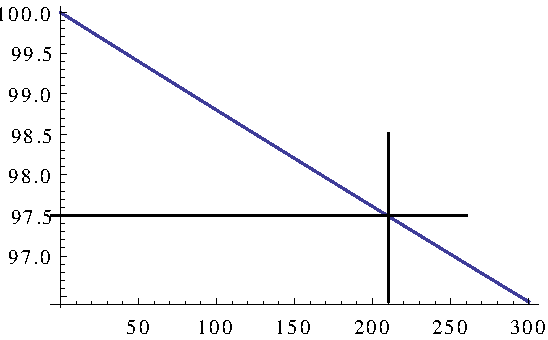
\includegraphics[width=\linewidth]{solutions/q2/q2plot.pdf}
\caption{Plot of carbon-14 decay over 300 years}
\label{fig:q2plot}
\end{figure} \\
Figure \ref{fig:q2plot} tells us the forgery was painted about 210 years ago.
For a more precise date we can solve for $t$ from (eq:\ref{eq:q2Simple}).
\begin{align}
  97.5 &= 100 \cdot e^{\frac{\ln\left(\frac{1}{2}\right)}{5730} \cdot t} \nonumber \\
  \frac{97.5}{100} &= e^{\frac{\ln\left(\frac{1}{2}\right)}{5730} \cdot t} \\
  \ln\left(\frac{97.5}{100} \right) &= \frac{\ln\left(\frac{1}{2}\right)}{5730} \cdot t \\
  \ln\left(\frac{97.5}{100} \right) \cdot \frac{5730}{\ln\left(\frac{1}{2}\right)} &= t \\
   &= 209.23...
\end{align}
209.23 years is close to the 210 year ball park for the age, putting the date of
painting at 1806. $\therefore$ the painting is a forgery $\because$ 1806 is well
after Bruegel's time. \qedbitches
